%% This is an example first chapter.  You should put chapter/appendix that you
%% write into a separate file, and add a line \include{yourfilename} to
%% main.tex, where `yourfilename.tex' is the name of the chapter/appendix file.
%% You can process specific files by typing their names in at the 
%% \files=
%% prompt when you run the file main.tex through LaTeX.
\chapter{Introduction}

A Disaster Management Information System (DMIS) can be a useful tool to extract data from social media platforms and parse information to save time during a crisis, which can mean life or death in such situations.

The subsequent chapters describe the literature, architecture and design of a disaster management system, and the motivations behind the design decisions made.

\section{Inspiration}

Disasters can strike without notice and no amount of preparation can compete with the knowledge to overcome the effects of a disaster during and after the incident. For example, a flash flood can happen with little to no warning and knowing safe zones during this disaster can help to save lives. The aim is to propose and implement a platform that can extract and store data from multiple social media platforms, news websites, and various other disaster-related data stores, and process this data to present valuable information in real-time.

The advent of digital age and resulting ever-connected society that shares localized information that was not available in the past has presented us with an opportunity to tap into these resources to gather very fine-tuned information of the incidents happening on the ground. Integrating this information in conjunction with the traditional ways of collecting data (e.g. Geo-spatial data, sensor data, satellite imagery) can provide better choices in decision making during a catastrophe.

\section{Leveraging existing data}

When disaster strikes, there's often no time to sift through data, much less try to analyze it. One way to avoid such a situation is to imagine all the possibilities of an emergency situation and line up the data beforehand. Unfortunately, that is not always possible, as you never know what data you will need until a situation occurs. The DMIS aims to do that by storing the needed information beforehand and processing the information so that it saves time during a disaster.

The storing of information and processing can be done since the abundance of data available on-line on Twitter and other social media platforms \cite{hristidis2010survey}. Websites like Twitter provide Application Programming Interfaces (APIs) to stream their data which can be filtered and saved in a database. The data can then be analyzed and filtered to gather useful information that can be acted upon.

\section{Scope of data collection} 

The mushrooming of social networking has made the general population inadvertently participate in data collection. This is comparable to having resources on the ground, providing access to information in real-time \cite{de2011use}.

The DMIS platform aims to collect data obtained from these sources on a streaming basis. Consequently, as the data is being obtained from a large pool of diverse information, the gathered data has to be specifically filtered for disaster-related information.

The information generated by the various participants can be classified into four disaster management phases, as illustrated in Figure 1.1: mitigation, preparedness, response, and recovery \cite{coppola2006introduction}. Mitigation involves the undertaking of steps to reduce the impact of a disaster on the loss of life and property before it occurs. This is done by meticulously planning infrastructures and strengthening them with additional efforts to make the community more resilient to catastrophic events. Preparedness is concerned with formulation of plans and protocols to follow during a disaster event. The goal is to be ready for a catastrophic event which includes developing response mechanisms, procedures, and strategies that can be adhered to during an event, while also educating the communities with these response mechanisms. In addition to these efforts, there is the setting up of warning systems, shelters and storing of reserves such as food, water, medicines and other equipment and essentials that will be needed during a crisis. 

\begin{figure}[ht!]
	\centering
	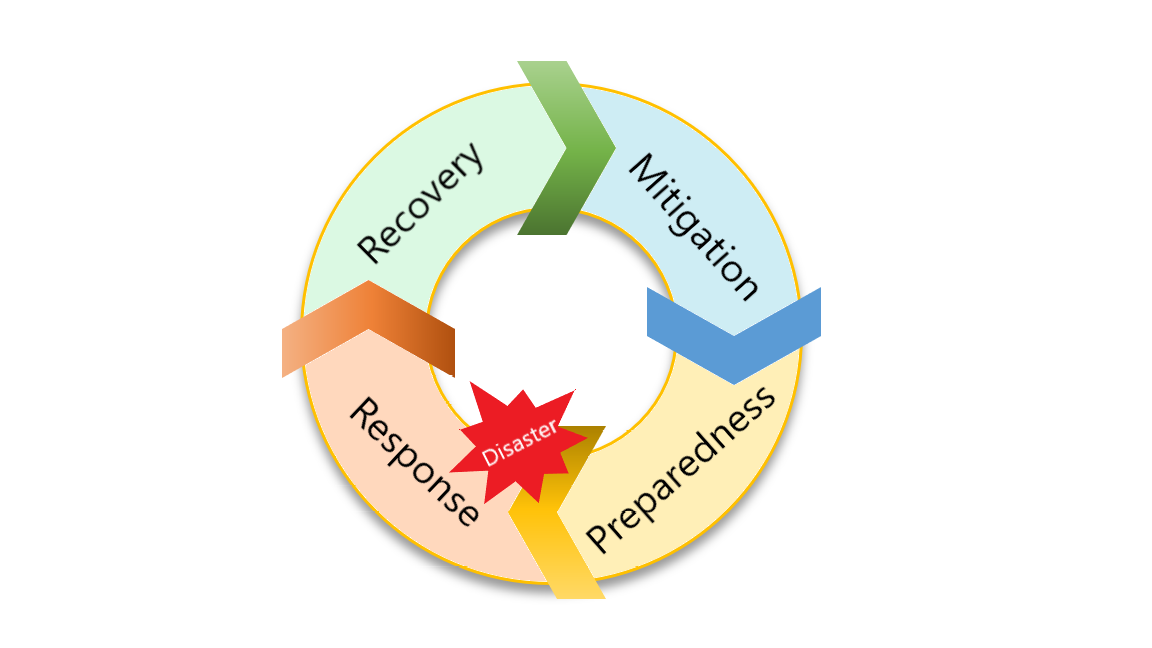
\includegraphics[width=150mm]{disaster.png}
	\caption{Phases of disaster management. \label{overflow}}
\end{figure}

The data during the mitigation and preparedness phases ranges from response plans, emergency procedures, records for training exercises, and available resources. The response phase is triggered when a catastrophe occurs. This phase deals with the immediate assistance to save lives and improve health and morale of the affected population. Assistance includes providing safe zones and shelters, preservation of property, and provides information such as places to avoid, evacuation plans, extraction zones and protocols to follow.

The aftermath of a disaster is when the recovery phase starts. This is done by providing assistance to bring normalcy back, including repairing of damaged structures, clearing of debris, helping to resume business operations and getting the population back on their feet. Examples of data generated during the response and recovery phases consists of incident reports, lessons learned and use of the resulting information to make better disaster plans.

The data generated during the response phase is very crucial and if this data is carefully extrapolated and presented in real-time, it can make a difference during an incident. The approach proposed in this study aims to deliver this data efficiently with solutions to various challenges arising in the development of the system. Additionally, the scope of the system encompasses to be a knowledge base before, during and after a disaster. This can done by collecting data during all the phases of the disaster but effectively delivering during the response phase.

\section{Glimpse into the system}

Recent advancements in cloud computing, Big Data and NoSQL databases as well as the rising popularity of data science, machine learning and deep learning techniques have changed how data is being captured, stored and analyzed. NoSQL solutions are especially popular in Web applications \cite{sakr2011survey}, that include Facebook, Twitter, and Google as well as popular news websites like CNN and New York Times. However, the usage of cloud computing technologies and NoSQL solutions in addition to data science algorithms have been not fully explored in solutions to a disaster management system.

Benefits of storing and analyzing disaster related data in a cloud environment can have advantages \cite{kossmann2010data} such as:

\begin{description}
	
	\item[$\bullet$ \it High Availaibility.]
	\hfill\break
	In a cloud environment the data is made redundant by using replication techniques where the data is stored in separate locations which are ofter geographically apart across large distances. This leads to data persistence even if a local data center fails as a switchover can occur almost instantaneously, resuming normal operation of the system without any delay.
	
	\item[$\bullet$ \it Scalability and elasticity.]
	\hfill\break
	The amount of data being captured can be massive, also the computational power required to process this data can also vary greatly at a particular time a cloud based solution can adapt storage and processing resources on demand based on real-time needs and priorities. Additionally the data can be distributed heterogeneously on servers that can be run in parallel to increase performance of the system.  
	
	\item[$\bullet$ \it Cost Effective.]
	\hfill\break
	The initial investment to start and running the system on a cloud platform can be minimal. Additionally the system can be expanded by adding new nodes as and when needed.
\end{description}

On the other hand there are many advantages of using NoSQL data stores for disaster data management, including:

\begin{description}
	
	\item[$\bullet$ \it Flexible data structure.]
	\hfill\break
	Since the data collection includes data from various sources this makes the disaster data extremely diverse making it challenging to store information in a predetermined data structure, NoSQL data stores make it possible to store a variety of data in the same database.
	
	\item[$\bullet$ \it Horizontal scalability.]
	\hfill\break
	NoSQL data stores were explicitly designed to handle large amounts of data by making it easy to scale on an as needed basis. This can be done easily by adding additional nodes to increase storage and handling.
	
	\item[$\bullet$ \it Performance.]
	\hfill\break
	NoSQL data stores are faster on simple read/write operations. They are designed to do parallel processing on different nodes compared to relational databases, giving them an edge in performance oriented applications.
\end{description}

The increase in popularity of data science techniques has demonstrated the power of building complex quantitative algorithms to organize and synthesize large amounts of information used to answer questions and develop strategies to tackle complex problems in faster and efficient way. Advantages to using data science to filter and analyze the data being stored include:

\begin{description}
	
	\item[$\bullet$ \it Faster processing.]
	\hfill\break
	Using machine learning algorithms based on proven statistical models the data processing can be speedy.
	
	\item[$\bullet$ \it Easy classification.]
	\hfill\break
	Sorting through the variety of the data being collected can be a daunting task as the data being stored is structured, semi-structured and unstructured.This data can be easily filtered by using classifiers, saving time and decreasing the overhead of searching through all the data in the data store.
\end{description}

\section{Thesis Structure}

The chapters in this thesis are organized as follows:

\begin{description}
	
	\item[$\bullet$ ]
	\textbf {Chapter 2} describes the concepts and technologies relevant to this study: Big Data, cloud computing, NoSQL data stores and Machine Learning. Big Data is introduced as the data is gathered and stored from diverse sources. Also, since the platform designed is cloud-based, the nature of cloud computing model is delved into. Next, the storage model incorporated in the system; NoSQL is introduced. Also, different data models are discussed in reference to DMIS platform. Finally, machine learning is introduced and its applications in DMIS.

	\item[$\bullet$ ]
	\textbf {Chapter 3} defines the DMIS platform, listing the specific technologies used to implement the platform. Here, data from twitter is streamed and stored as 'proof of concept'. Next, the filtering techniques are described. Finally, the cloud based platform used to host the platform is introduced.

	\item[$\bullet$ ]
	\textbf {Chapter 4} concludes this study by discussing the contributions of this research. The main contribution is the implementation of the Disaster Information Management System as an information delivery service. The implementation is generic and can be used in other domains.

	\item[$\bullet$ ]
	\textbf {Chapter 5} focuses on the future aspects of the system, such as the potential of expanding of the system to increase the reach by creating portable and platform specific applications. Further work also includes working on data filtering techniques, verifying the data authenticity, etc.

\end{description}

% This is an example of how you would use tgrind to include an example
% of source code; it is commented out in this template since the code
% example file does not exist.  To use it, you need to remove the '%' on the
% beginning of the line, and insert your own information in the call.
%
%\tagrind[htbp]{code/pmn.s.tex}{Post Multiply Normalization}{opt:pmn}


% This is an example of how you would use tgrind to include an example
% of source code; it is commented out in this template since the code
% example file does not exist.  To use it, you need to remove the '%' on the
% beginning of the line, and insert your own information in the call.
%
%\tgrind[htbp]{code/be.s.tex}{Block Exponent}{opt:be}
